\documentclass[a4paper, 11pt]{report}%{spie}
%\usepackage[latin1]{inputenc} accents under Linux/Unix
%\usepackage[applemac]{inputenc} %accents under MacOS 
%\usepackage[ansinew]{inputenc} accents under Windows
\usepackage[utf8]{inputenc} %accents under any OS but in TeXShop, requieres preferences/encoding to be set on UTF-8 BEFORE creating the document
\usepackage[english]{babel}

\usepackage{geometry}                % See geometry.pdf to learn the layout options. There are lots.
%\geometry{letterpaper}                   % ... or a4paper or a5paper or ... 
%\geometry{landscape}                % Activate for for rotated page geometry
%\usepackage[parfill]{parskip}    % Activate to begin paragraphs with an empty line rather than an indent
\usepackage{graphicx, mdwlist}
\usepackage{amssymb}
\usepackage{epstopdf}
\usepackage{verbatim}

\usepackage{hyperref}
\hypersetup{ 
     backref=true,    %permet d'ajouter des liens dans... 
     pagebackref=true,%...les bibliographies 
     hyperindex=true, %ajoute des liens dans les index. 
     colorlinks=true, %colorise les liens 
     breaklinks=true, %permet le retour à la ligne dans les liens trop longs 
     urlcolor= blue,  %couleur des hyperliens 
     linkcolor= blue, %couleur des liens internes 
     bookmarks=true,  %créé des signets pour Acrobat 
     bookmarksopen=true,            %si les signets Acrobat sont créés, les afficher complètement. 
} 

\usepackage{pdftricks}
\begin{psinputs}
   \usepackage{pstricks}
   \usepackage{pst-node}
\end{psinputs}

\usepackage[version=3]{mhchem}
\usepackage[makeroom]{cancel}
\usepackage{moresize}

\DeclareGraphicsRule{.tif}{png}{.png}{`convert #1 `dirname #1`/`basename #1 .tif`.png}
\pagestyle{plain}

\newcommand{\mailbug}{\begin{center}\textbf{To report any bug you may find while using this plugin, \href{mailto:fabrice.cordelieres@gmail.com,cedric.matthews@ibdml.univ-mrs.fr ?subject=Bug\%20found\%20in\%20MetroloJ&body=\%0ABug\%20description:\%0A\%0AHow\%20did\%20it\%20happen:\%0A\%0ACopy/Paste\%20the\%20content\%20of\%20the\%20log\%20window\%0A\%0AVersion\%20of\%20ImageJ:\%0A\%0AVersion\%20of\%20Java:}{please click here}}.\end{center}}


\title{
\textbf{The MetroloJ plugin}}
\author{\href{mailto:fabrice.cordelieres@gmail.com}{Fabrice P. Cordelières}, \href{mailto:cedric.matthews@ibdml.univ-mrs.fr }{Cédric Matthews}
\date{\today}        % Activate to display a given date or no date
}


%%%%%%%%%%%%%%%%%%%%%%%%%%%%%%%%%%%%%%%%%%%%%%%%%%%%%%%%%%%%%
\begin{document}

\begin{table}[!t]
	\begin {center}
			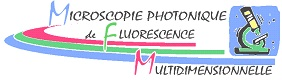
\includegraphics[width=0.35\linewidth]{img/logo_RT-MFM}  \hfill 
\includegraphics[width=0.25\linewidth]{img/logo_mrct}
	\end {center}
\end{table}

\maketitle

\newpage

\tableofcontents

\newpage

\begin{flushright}
\section*{}
\textit{This manual and plugin comes as a result of a collective work of the ``Metrology group'' within the \href{http://rtmfm.ibl.fr/}{French Technological Network of the Multi-Dimensional Fluorescence Microscopies (RT-MFM)}, supported by the \href{http://www.mrct.cnrs.fr/}{``Mission Ressources et Compétences Technologiques'' (MRCT)}.\\
\vspace{0.5cm}
The authors would like to thank:\\
Aurélie Le Ru for reporting the time-shift bug.\\
Fran\c cois Waharte for beta-testing and bug tracking.\\
Claude-Marie Bachelet and Aurélien Dauphin for the images used in fig. \ref{fig:gcoar-report}\\
Aude Jobart for images of spinning disc PSFs\\
\vspace{0.5cm}
}

\textit{We would like to acknowledge the work of all the valuable beta-tester and the member of the ``groupe de travail Métrologie du RT-MFM'' who made feedback on the plugins collection and helped us improving and adapting it:\\
Pierre Bourdoncle, Anne Cantereau, Julien Cau, Christophe Chamot, Julien Cianfichi, 
Aurélien Dauphin, Olivier Duc, Sylvain De Rossi, Stéphanie Dutertre, Aude Jobart-Malfait, Christophe Klein, Marc Lartaud, Patricia Le Baccon, Aurélie Le Ru, Meriem Garfa-Traoré, Camille Lebugle, Sandrine Leveque-Fort, Christophe Machu, Laure Malicieux, Christel Poujol, Richard Schwartzmann, Damien Schapman, Marie-Noëlle Soler, Nicolas Tissot, Yves Usson and Fran\c cois Waharte.
}
\end{flushright}
\newpage

%%%%%%%%%%%%%%%%%%%%%%%%%%%%%%%%%%%%%%%%%%%%%%%%%%%%%%%%%%%%%
\chapter{How to install the plugin ?}

First, close ImageJ in case the software is already running. Copy and paste the \textit{\textbf{MetroloJ.jar}} file into the ImageJ/Plugins folder. Download the \textit{\textbf{iText library}} by following \href{http://prdownloads.sourceforge.net/itext/iText-2.1.5.jar}{this link}. This library will be used by the plugin to generate pdf reports. Copy and paste it into the ImageJ/Plugins folder. Restart ImageJ.\\
A \textit{\textbf{MetroloJ}} entry should appear under the ImageJ's plugins menu. It contains 2 entries:

\begin{itemize*} % mdwlist defines enumerate*, & itemize* to create COMPACT listings
	\item \htmlref{Generate PSF report}{chap:gpr};
	\item \htmlref{Generate co-alignement report}{chap:gcoar};.
\end{itemize*}

\mailbug

%%%%%%%%%%%%%%%%%%%%%%%%%%%%%%%%%%%%%%%%%%%%%%%%%%%%%%%%%%%%%
\chapter{Generate CV report}
\label{chap:gcvr}

%--------------------------------------------------------------------------------------------------------------------------------------------------------------------
\section{How to generate the images ?}
\label{sec:gcvr-what}

\subsection{How to prepare the sample ?}
\label{sec:gcvr-proto}

\textit{There is no real sample preparation, the only required material is detailed here after.}

\subsubsection{What do I need ?}
\label{sec:gcvr-proto-what}

\begin{itemize*}
	\item \textbf{\textit{Fluorescent slides:}} made of fluorescent plastic, the fluorescent slide provides the user with a uniformly labelled sample. They might be ordered from \href{https://www.omegafilters.com/index.php?page=prod_rslides_pro}{Omega Opticals} or \href{http://www.microscopyeducation.com/fluorrefslides.html}{Microscopy Education}.
	\item \textbf{\textit{Alternatively}}, large diameter uniformly labelled beads might also be used and prepared as explained under the ``Generate co-alignement report'' section (\ref{sec:gcoar-proto-what}).
\end{itemize*}

\subsection{How to acquire the image ?}
\label{sec:gcvr-flow}

The following chart (see fig. \ref{fig:gcvr-flowImg}) summarizes the procedure for optimal image acquisition, in order to determine the CV of several PMTs on a confocal microscope.

\begin{figure}
	\begin{pdfpic}
		\begin{psmatrix}[colsep=0.4,rowsep=0.3075]
			[name=1] \psovalbox[fillstyle=solid, fillcolor=yellow, shadow=true]{\textbf{Begin}}\\
			[name=2] \psframebox[shadow=true]{Set the scanning mode to XYZ}\\
			[name=3] \psframebox[shadow=true]{Set the zoom to reach a proper sampling rate}\\
			[name=4] \psframebox[shadow=true]{Adjust the laser output to its minimum}\\
			[name=5] \psframebox[shadow=true]{Adjust z position}\\
			[name=6] \psdiabox[fillstyle=solid, fillcolor=lightgray, shadow=true]{\begin{tabular}{c}Surface of the\\slide found ?\end{tabular}}\\\\
			[name=7]  \psframebox[shadow=true]{Adjust the gain for all PMTs}\\
			[name=8] \psdiabox[fillstyle=solid, fillcolor=lightgray,shadow=true]{\begin{tabular}{c}Images close\\to saturation ?\end{tabular}}\\\\
			[name=9] \psframebox[shadow=true]{Set the acquisition averaging to 1}\\
			[name=10] \psframebox[shadow=true]{Acquire the images (one per PMT)}\\
			[name=11] \psframebox[shadow=true]{Generate the report using MetroloJ}\\
			[name=12] \psovalbox[fillstyle=solid, fillcolor=yellow, shadow=true]{\textbf{End}}
		
			\ncline{->}{1}{2}
			\ncline{->}{2}{3}
			\ncline{->}{3}{4}
			\ncline{->}{4}{5}
			\ncline{->}{5}{6}
			\ncangles[loopsize=1, arm=.5]{->}{6}{5} \aput{:U}{\textbf{No}}
			\ncline{->}{6}{7}\aput{:U}{\textbf{Yes}} 
			\ncline{->}{7}{8}
			\ncangles[loopsize=1, arm=.5]{->}{8}{7} \aput{:U}{\textbf{No}}
			\ncline{->}{8}{9} \aput{:U}{\textbf{Yes}} 
			\ncline{->}{9}{10}
			\ncline{->}{10}{11}
			\ncline{->}{11}{12}
		\end{psmatrix}
	\end{pdfpic}
	\caption{\label{fig:gcvr-flowImg}Acquisition of the images for CV measurement (confocal).}
\end{figure}

\newpage

%--------------------------------------------------------------------------------------------------------------------------------------------------------------------
\section{What does it do ?}
\label{sec:gcvr-what}

\begin{enumerate*}
	\item The plugin measures the average intensity ($\mu$) and the standard deviation ($\sigma$) of the gray levels within a user defined region of interest (ROI) for each image of a stack corresponding to acquisitions made for each PMT to compare.
	\item It calculates the coefficient of variation (CV) as follows:
		\begin{equation}
			CV = \frac{\sigma}{\mu}
			\label{eqn:gcvr-CV}
		\end{equation}
	\item The normalized CV is then calculated as the ratio of the current image's CV over the minimum retrieved CV over all images.
\end{enumerate*}

%--------------------------------------------------------------------------------------------------------------------------------------------------------------------
\section{How to use it ?}
\label{sec:gcvr-how}

\begin{enumerate*}
	\item Start ImageJ;
	\item Open a stack of images containing the acquisitions made with the PMTs to analyze;
	\item Launch the plugin by going to Plugins/MetroloJ/Generate CV report
	\item In case the image has not been spatially calibrated, a message error pops up: click on Ok. In the calibration dialog box provide the appropriate values, then re-launch the plugin;
	\item The plugin's interface should appear (see fig. \ref{fig:gcvr-interf}); 
		\begin{figure}[!ht]
			\begin{center}
				\begin{tabular}{c}
					%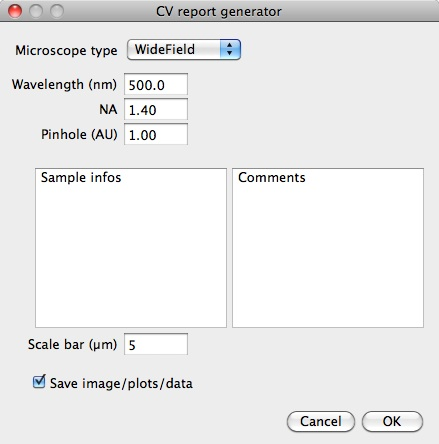
\includegraphics[width=0.35\linewidth]{img/gcvr-interf}
				\end{tabular}
			\end{center}
			\caption{\label{fig:gfir-interf}Generate CV report: the interface.}
		\end{figure} 
	\item Choose the microscope's type, enter the emission wavelength, the numerical aperture of the objective and the pinhole aperture. Sample informations and some comments might also be provided using the appropriate boxes. Ticking the ``Save image/plots/data'' will generate:
	\begin{itemize*}
		\item a jpeg panel containing all the analyzed images overlayed with the user defined ROIs;
		\item a jpeg image of the intensity distribution (histogram) for each image, within the user defined ROIs;
		\item a zip file containing the user defined ROIs;
		\item two files containing tabulation separated values of the histograms, and for the data used to calculate the raw and normalized CVs (excel files);
	\end{itemize*}
	\item Click on Ok: a new dialog box appears, inviting the user to choose a folder where all data will be saved;
	\item The pdf report is generated, and appropriate files saved.
\end{enumerate*}

%--------------------------------------------------------------------------------------------------------------------------------------------------------------------
\section{What's on the report ?}
\label{sec:gcvr-rep}

The CV report is composed of two pages (see an example of report on fig. \ref{fig:gcvr-report}) based on the informations provided by the user. It is composed of up to 6 sections:
\begin{figure}[!ht]
		\begin{center}
		\begin{tabular}{c}
			%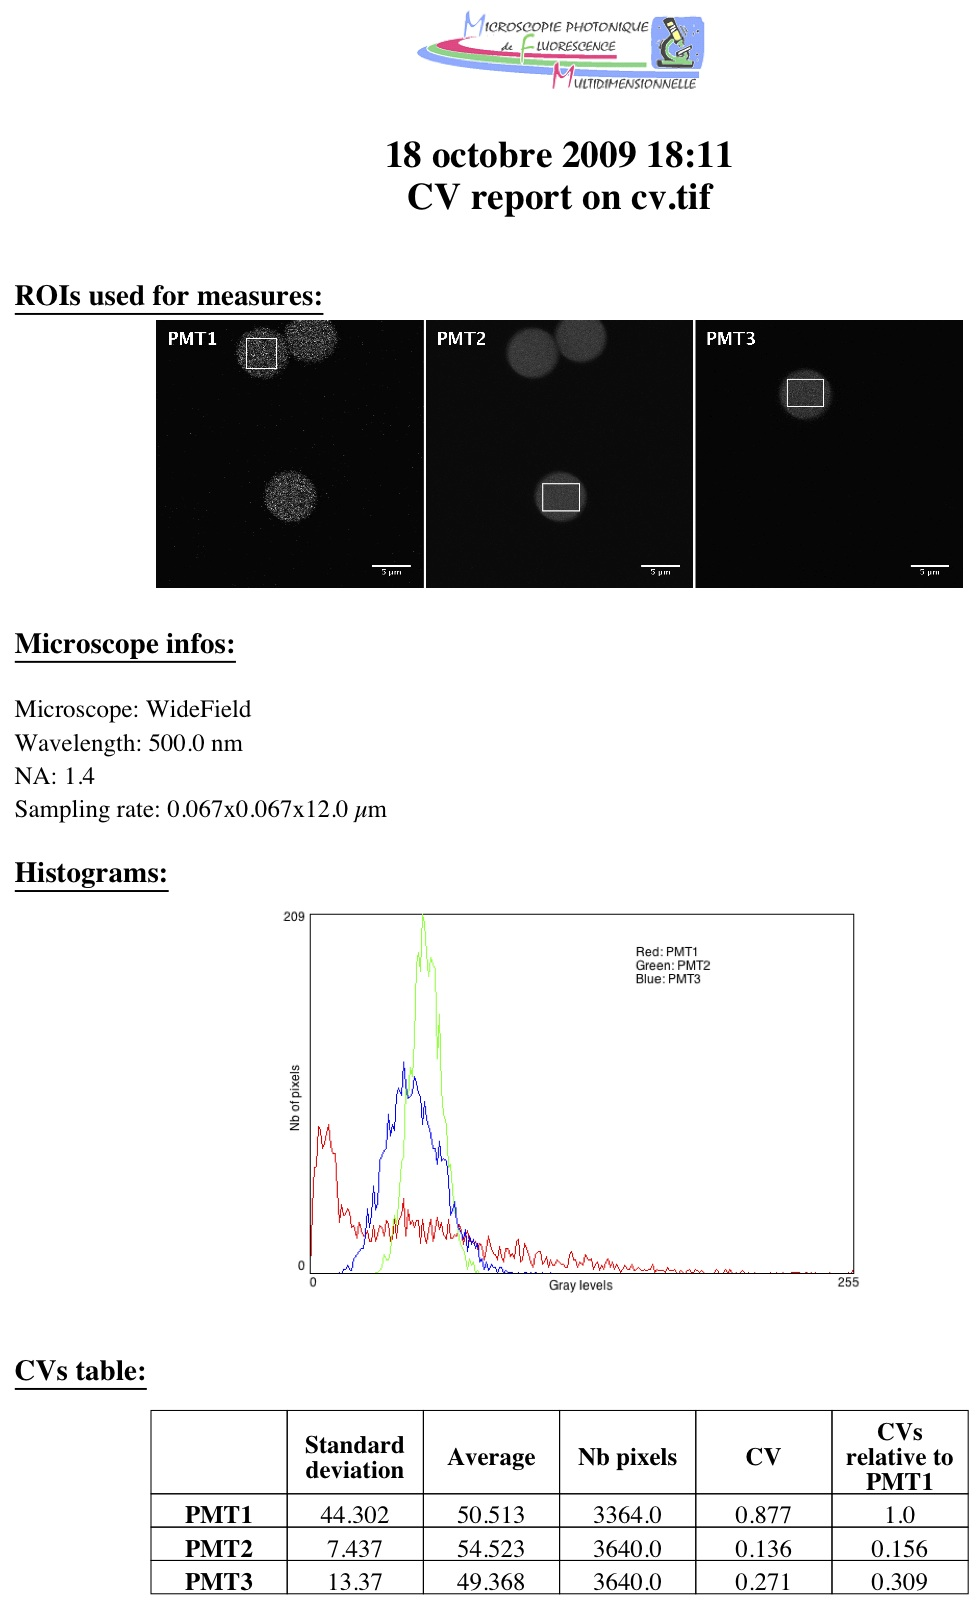
\includegraphics[width=\linewidth]{img/gcvr-report}
		\end{tabular}
	\end{center}
	\caption{\label{fig:gcvr-report}Generate CV report: an example of report.}
\end{figure} 
\begin{itemize*}
	\item \textbf{\textit{ROIs used for measures}}: montage composed of the images acquires using each PMT, overlayed with the user defined ROIs used for measurements;
	\item \textbf{\textit{Microscope infos}}: summarizes informations about the acquisition system and the image's calibration;
	\item \textbf{\textit{Histograms}}: plot of the gray level distributions within the user defined ROIs for each image;
	\item \textbf{\textit{CVs table}}: contains for each image the $\mu$ and $\sigma$ values, as well as the ROI size (expressed in number of pixels), the raw and normalized CVs;
	\item \textbf{\textit{Sample infos (optional)}}: contains the informations entered by the user in the ``Sample infos'' section of the interface;
	\item \textbf{\textit{Comments (optional)}}: contains the informations entered by the user in the ``Comments'' section of the interface;
\end{itemize*}

%--------------------------------------------------------------------------------------------------------------------------------------------------------------------
\section{Known issues (to date...) and workarounds (if any...)}
\label{sec:gcvr-ki}

None...yet.

\mailbug

%%%%%%%%%%%%%%%%%%%%%%%%%%%%%%%%%%%%%%%%%%%%%%%%%%%%%%%%%%%%%
\chapter{Generate field illumination report}
\label{chap:gfir}

%--------------------------------------------------------------------------------------------------------------------------------------------------------------------
\section{How to generate the images ?}
\label{sec:gfir-what}

\subsection{How to prepare the sample ?}
\label{sec:gfir-proto}

\textit{There is no real sample preparation, the only required material is detailed here after.}

\subsubsection{What do I need ?}
\label{sec:gfir-proto-what}

\begin{itemize*}
	\item \textbf{\textit{Fluorescent slides:}} made of fluorescent plastic, the fluorescent slide provides the user with a uniformly labelled sample. They might be ordered from \href{https://www.omegafilters.com/index.php?page=prod_rslides_pro}{Omega Opticals} or \href{http://www.microscopyeducation.com/fluorrefslides.html}{Microscopy Education}.
\end{itemize*}

\subsection{How to acquire the image ?}
\label{sec:gfir-flow}

The following chart (see fig. \ref{fig:gfir-flowImg}) summarises the procedure for optimal image acquisition, in order to determine field illumination homogeneity on a confocal microscope.

\begin{figure}
	\begin{pdfpic}
		\begin{psmatrix}[colsep=0.4,rowsep=0.3075]
			[name=1] \psovalbox[fillstyle=solid, fillcolor=yellow, shadow=true]{\textbf{Begin}}\\
			[name=2] \psframebox[shadow=true]{Set the scanning mode to XYZ}\\
			[name=3] \psframebox[shadow=true]{Set the zoom to reach a proper sampling rate}\\
			[name=4] \psframebox[shadow=true]{Adjust the laser output to its minimum}\\
			[name=5] \psframebox[shadow=true]{Adjust z position}\\
			[name=6] \psdiabox[fillstyle=solid, fillcolor=lightgray, shadow=true]{\begin{tabular}{c}Surface of the\\slide found ?\end{tabular}}\\\\
			[name=7]  \psframebox[shadow=true]{Adjust PMT's gain}\\
			[name=8] \psdiabox[fillstyle=solid, fillcolor=lightgray,shadow=true]{\begin{tabular}{c}Image close\\to saturation ?\end{tabular}}\\\\
			[name=9] \psframebox[shadow=true]{Set the acquisition averaging to 2-4}\\
			[name=10] \psframebox[shadow=true]{Acquire the image}\\
			[name=11] \psframebox[shadow=true]{Generate the report using MetroloJ}\\
			[name=12] \psovalbox[fillstyle=solid, fillcolor=yellow, shadow=true]{\textbf{End}}
		
			\ncline{->}{1}{2}
			\ncline{->}{2}{3}
			\ncline{->}{3}{4}
			\ncline{->}{4}{5}
			\ncline{->}{5}{6}
			\ncangles[loopsize=1, arm=.5]{->}{6}{5} \aput{:U}{\textbf{No}}
			\ncline{->}{6}{7}\aput{:U}{\textbf{Yes}} 
			\ncline{->}{7}{8}
			\ncangles[loopsize=1, arm=.5]{->}{8}{7} \aput{:U}{\textbf{No}}
			\ncline{->}{8}{9} \aput{:U}{\textbf{Yes}} 
			\ncline{->}{9}{10}
			\ncline{->}{10}{11}
			\ncline{->}{11}{12}
		\end{psmatrix}
	\end{pdfpic}
	\caption{\label{fig:gfir-flowImg}Acquisition of the image of a field to determine illumination's homogeneity (confocal).}
\end{figure}

\newpage

%--------------------------------------------------------------------------------------------------------------------------------------------------------------------
\section{What does it do ?}
\label{sec:gfir-what}

\begin{enumerate*}
	\item The plugin generates a normalized view of the image. Its maximum intensity pixel being set to 100\%, an iso-intensity map is drawn, the intensity step between two successive areas being set by user.
	\item The maximum intensity pixel coordinates, the image barycenter's coordinates and the barycenter of the 100\% region are retrieved.
	\item From the input image, the plugin will generate and analyze four intensity profiles along the horizontal and vertical axis and both diagonals passing through the image's center.
	\item Raw and normalized intensities of 8 characteristic pixels, corresponding to the 8 intercepts of the lines along which the intensity profiles are retrieved, are determined.
\end{enumerate*}

%--------------------------------------------------------------------------------------------------------------------------------------------------------------------
\section{How to use it ?}
\label{sec:gfir-how}

\begin{enumerate*}
	\item Start ImageJ;
	\item Open an image containing the field illumination to analyze;
	\item Launch the plugin by going to Plugins/MetroloJ/Generate field illumination report
	\item In case the image has not been spatially calibrated, a message error pops up: click on Ok. In the calibration dialog box provide the appropriate values, then re-launch the plugin;
	\item The plugin's interface should appear (see fig. \ref{fig:gfir-interf}); 
		\begin{figure}[!ht]
			\begin{center}
				\begin{tabular}{c}
					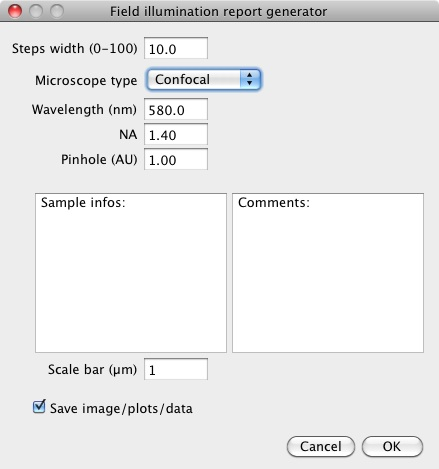
\includegraphics[width=0.35\linewidth]{img/gfir-interf}
				\end{tabular}
			\end{center}
			\caption{\label{fig:gfir-interf}Generate field illumination report: the interface.}
		\end{figure} 
	\item Choose the microscope's type, enter the emission wavelength, the numerical aperture of the objective and the pinhole aperture. Sample informations and some comments might also be provided using the appropriate boxes. Ticking the ``Save image/plots/data'' will generate:
	\begin{itemize*}
		\item a jpeg image of the illumination pattern;
		\item a jpeg image of the intensity profiles;
		\item two files containing tabulation separated values of the intensity profiles, and for the profiles associated statistics (excel files);
	\end{itemize*}
	\item Click on Ok: a new dialog box appears, inviting the user to choose a folder where all data will be saved;
	\item The pdf report is generated, and appropriate files saved.
\end{enumerate*}

%--------------------------------------------------------------------------------------------------------------------------------------------------------------------
\section{What's on the report ?}
\label{sec:gfir-rep}

The field illumination report is composed of two pages (see an example of report on fig. \ref{fig:gfir-report}) based on the informations provided by the user. It is composed of up to 6 sections:
\begin{figure}[!ht]
		\begin{center}
		\begin{tabular}{c}
			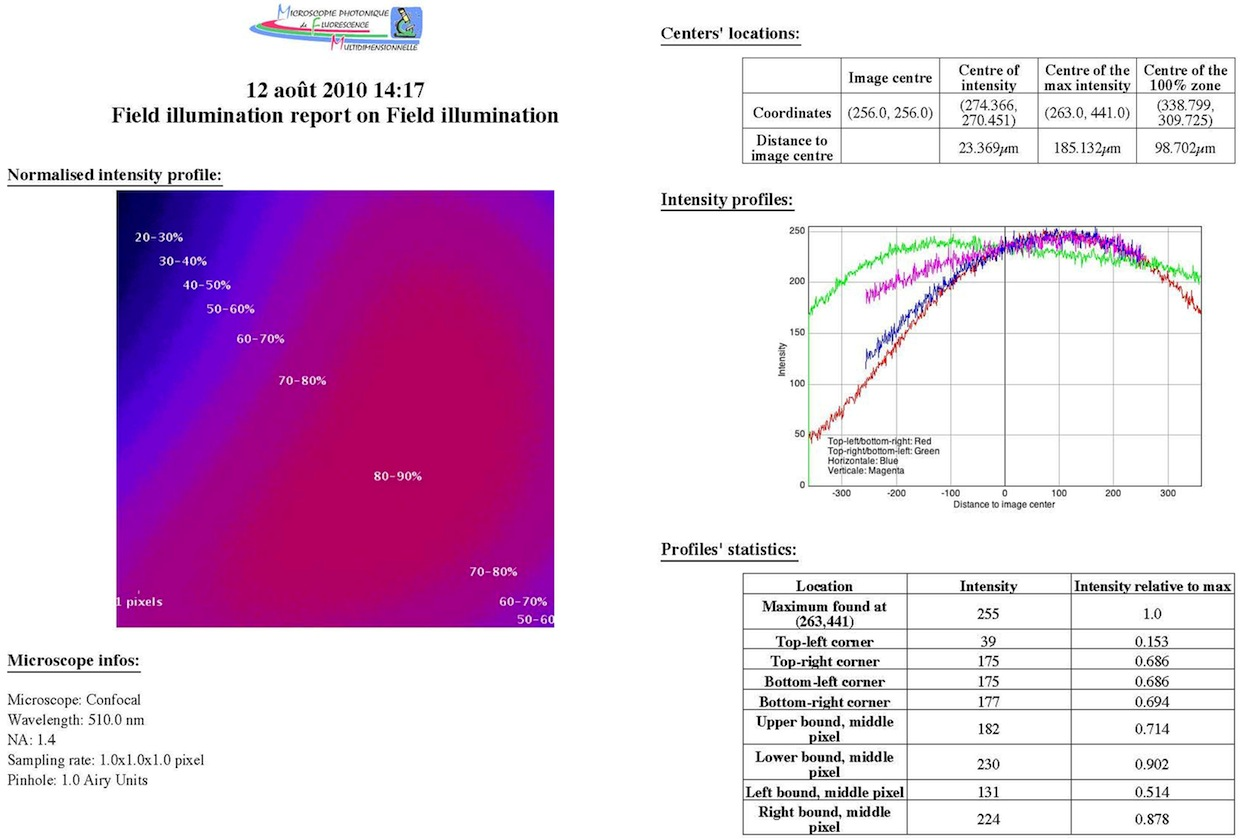
\includegraphics[width=\linewidth]{img/gfir-report}
		\end{tabular}
	\end{center}
	\caption{\label{fig:gfir-report}Generate field illumination report: an example of report.}
\end{figure} 
\begin{itemize*}
	\item \textbf{\textit{Normalized intensity profile}}: normalized view of the field illumination, in false color, separated into iso-intensity zones which step width is user defined;
	\item \textbf{\textit{Microscope infos}}: summarizes informations about the acquisition system and the image's calibration;
	\item \textbf{\textit{Centers' location}}: contains the coordinates of points of interest: the image center, the centre of intensity, the center of maximum intensity and the centre of the 100\% zone. It also displays the distances between the 3 later and the image's geometrical center;
	\item \textbf{\textit{Intensity profiles}}: contains a plot of the intensity profiles along the the horizontal and vertical axis and both diagonals passing through the image's center;
	\item \textbf{\textit{Profiles' statistics}}: contains both raw and normalized intensities of 8 characteristic pixels, corresponding to the 8 intercepts of the lines along which the intensity profiles are retrieved;
	\item \textbf{\textit{Sample infos (optional)}}: contains the informations entered by the user in the ``Sample infos'' section of the interface;
	\item \textbf{\textit{Comments (optional)}}: contains the informations entered by the user in the ``Comments'' section of the interface;
\end{itemize*}

%--------------------------------------------------------------------------------------------------------------------------------------------------------------------
\section{Known issues (to date...) and workarounds (if any...)}
\label{sec:gfir-ki}

None...yet.

\mailbug

%%%%%%%%%%%%%%%%%%%%%%%%%%%%%%%%%%%%%%%%%%%%%%%%%%%%%%%%%%%%%
\chapter{Generate PSF report}
\label{chap:gpr}

%--------------------------------------------------------------------------------------------------------------------------------------------------------------------
\section{How to generate the images ?}
\label{sec:gpr-what}

\subsection{How to prepare the sample ?}
\label{sec:gpr-proto}

\textit{This sample preparation is aimed at obtaining an array of fluorescent beads, well appart one from the other, and stably stuck to a coverslip.}

\subsubsection{What do I need ?}
\label{sec:gpr-proto-what}

\begin{itemize*}
	\item \textbf{\textit{Fluorescent beads:}} their outer diameter should be below the resolution of the system to test. Two types of beads might be used:
		\begin{itemize*}
			\item Mono-labelled beads. ex: Molecular Probes' \href{http://probes.invitrogen.com/media/pis/mp07220.pdf}{PS-Speck, Ref. P-7220}. However, their diameter of 0.17$\mu$m is a bit high for high NA objectives...
			\item Multi-labelled beads. ex: Molecular Probes' \href{http://probes.invitrogen.com/media/pis/mp07279.pdf}{TetraSpeck, Ref. T-7279}. Their diameter of 0.1$\mu$m is ideal, though having multi-labelled beads may lead to weaker signals...
		\end{itemize*}
	\item \textbf{\textit{Regular slides}};
	\item \textbf{\textit{Regular coverslips}}: type 1.5 i.e. 0.17mm thick, either polylysine coated or not;
	\item If applicable, \textbf{\textit{Poly-L-lysine solution}} (0.1 \% (w/v) in $H_{2}O$) ex: \href{http://www.sigmaaldrich.com/etc/medialib/docs/Sigma/generalinformation2/p8920.Par.0001.File.tmp/p8920.pdf}{Sigma-Aldrich, Ref. P8920};
	\item \textbf{\textit{Ethanol}};
	\item \textbf{\textit{Regular distilled water}};
	\item \textbf{\textit{Mounting medium}}: should be the same as for the regular, biological samples. Avoid using DAPI containing mounting media;
	\item \textbf{\textit{Nail polish}}: only in case the mounting solution is not a setting medium.
\end{itemize*}

\subsubsection{How do I do ?}
\label{sec:gpr-proto-how}

\begin{enumerate*}
	\item Clean the coverslip and the slide using ethanol;
	\item Dilute the polylysine stock solution to 1/5$^{th}$;
	\item Poor a sufficient amount of the diluted polylysine solution onto the coverslip surface (typically, 200$\mu$l for a 24x24mm coverslip) and leave to coat for 15-30 minutes. The solution hardly covers the full surface, so don't hesitate to use the pipet's tip to force the polylysine into the coverslip's corners; 
	\item Rince the coverslip 2-3 times in distilled water, then drain off the liquid;
	\item Use a vortex to mix the beads' stock suspension;
	\item Dilute the beads suspension in water. Here are some tips and facts:
		\begin{itemize*}
			\item Typically, 200$\mu$l for a 24x24mm coverslip will be requiered;
			\item In general, the 0.1$\mu$m \href{http://probes.invitrogen.com/media/pis/mp07279.pdf}{TetraSpeck} should be diluted to 1/1,000, the \href{http://probes.invitrogen.com/media/pis/mp07220.pdf}{PS-Speck} from 1/10,000 to 1/40,000;
			\item It is advised to first dilute the beads to 1/1,000, then make further serial dilution to achieve the appropriate beads' density on slide.
			\item Tests should be done to define the appropriate dilution ratio;
			\item Always vortex the suspensions between and after dilutions;
		\end{itemize*}
	\item Poor a sufficient amount of the diluted beads suspension onto the coverslip surface and leave to sediment for at least 30 minutes. The solution hardly covers the full surface, so don't hesitate to use the pipet's tip to force the suspension into the coverslip's corners; 
	\item Rince the coverslip 2-3 times in distilled water to remove the unattached beads, then drain off the liquid;
	\item Mount the coverslip on the slide by using the mounting medium. In case of non setting media, the coverslip should be sealed onto the slide using nail polish, while avoiding the latter to come under the coverslip.
\end{enumerate*}

NB: Other methods exists in order to produce beads slides, involving dilution in ethanol and leaving the suspension to evaporate. In this case, tests of higher beads dilution might be required. Please note that already prepared beads slides are commercially available (see \href{http://probes.invitrogen.com/media/pis/mp07279.pdf}{TetraSpeck Fluorescent Microspheres Size Kit mounted on slide}). However, this kind of preparation doesn't always match with the real \textit{in situ} resolution as the mounting medium might be different from the one used in everyday acquisitions.

\subsection{How to acquire the image ?}
\label{sec:gpr-flow}

The following chart (see fig. \ref{fig:gpr-flowImg}) summarises the procedure for optimal image acquisition, in order to determine the resolutions on a confocal microscope.

\begin{figure}
	\begin{pdfpic}
		\begin{psmatrix}[colsep=0.4,rowsep=0.3075]
			[name=1] \psovalbox[fillstyle=solid, fillcolor=yellow, shadow=true]{\textbf{Begin}}\\
			[name=2] \psframebox[shadow=true]{Set the scanning mode to XYZ}\\
			[name=3] \psframebox[shadow=true]{Set the zoom to reach a slight oversampling rate}\\
			[name=4] \psframebox[shadow=true]{Adjust the laser output to its minimum}\\
			[name=5] \psframebox[shadow=true]{Adjust z position}\\
			[name=6] \psdiabox[fillstyle=solid, fillcolor=lightgray, shadow=true]{\begin{tabular}{c}Centre of the\\bead found ?\end{tabular}}\\\\
			[name=7] \psframebox[shadow=true]{Adjust xy position}\\
			[name=8] \psdiabox[fillstyle=solid, fillcolor=lightgray, shadow=true]{\begin{tabular}{c}Centre well\\centred on pixels ?\end{tabular}}\\\\
			[name=9] \psframebox[shadow=true]{Set the acquisition's top and bottom}\\
			[name=10] \psframebox[shadow=true]{Adjust PMT's gain}\\
			[name=11] \psdiabox[fillstyle=solid, fillcolor=lightgray,shadow=true]{\begin{tabular}{c}Image's centre close\\to saturation ?\end{tabular}}\\\\
			[name=12] \psframebox[shadow=true]{Set the acquisition averaging to 2-4}\\
			[name=13] \psframebox[shadow=true]{Acquire the stack}\\
			[name=14] \psframebox[shadow=true]{Generate the report using MetroloJ}\\
			[name=15] \psovalbox[fillstyle=solid, fillcolor=yellow, shadow=true]{\textbf{End}}
		
			\ncline{->}{1}{2}
			\ncline{->}{2}{3}
			\ncline{->}{3}{4}
			\ncline{->}{4}{5}
			\ncline{->}{5}{6}
			\ncangles[loopsize=1, arm=.5]{->}{6}{5} \aput{:U}{\textbf{No}}
			\ncline{->}{6}{7}\aput{:U}{\textbf{Yes}} 
			\ncline{->}{7}{8}
			\ncangles[loopsize=1, arm=.5]{->}{8}{7} \aput{:U}{\textbf{No}}
			\ncline{->}{8}{9} \aput{:U}{\textbf{Yes}} 
			\ncline{->}{9}{10}
			\ncline{->}{10}{11}
			\ncangles[loopsize=1, arm=.5]{->}{11}{10} \aput{:U}{\textbf{No}}
			\ncline{->}{11}{12}\aput{:U}{\textbf{Yes}}
			\ncline{->}{12}{13}
			\ncline{->}{13}{14}
			\ncline{->}{14}{15}
		\end{psmatrix}
	\end{pdfpic}
	\caption{\label{fig:gpr-flowImg}Acquisition of the image of a PSF for resolutions determination (confocal).}
\end{figure}

\newpage

%--------------------------------------------------------------------------------------------------------------------------------------------------------------------
\section{What does it do ?}
\label{sec:gpr-what}

\begin{enumerate*}
	\item The plugin will generate a maximum intensity projection of the stack along the z axis. The (x, y) coordinates of the maximum intensity pixel (MIPix) are then collected. A XZ cross-section is generated, along a line passing through the previously determined 2D MIPix. From this image, the z coordinate of the MIPix is defined.
	\item The z slice is set to the z MIPix coordinate. The x profile and y profile are collected along the line passing through the MIPix. The z profile is collected on the XZ view, along the line passing through the MIPix.
	\item All three profiles are fitted to a Gaussian, using the following equation and ImageJ's built-in curve fitting function:
		\begin{equation}
			y = a + (b-a)*e^{\frac{-(x-c)^{2}}{2*d^{2}}}
			\label{eqn:gpr-gaussian}
		\end{equation}
	\item The resolution i.e. the full-width at half-maximum (FWHM) is calculated as follows for each profile, based on the parameters retrieved from the fitting:
	\begin{equation}
		FWHM=2d\sqrt{2ln(2)}
		\label{eqn:gpr-FWHM}
	\end{equation}
	\item The theoretical resolutions are calculated as follows, depending on the microscope's type:
		\begin{eqnarray}
			xy_{resol, wide-field}=\frac{0.61*\lambda_{emission}}{NA}
			\label{eqn:gpr-xyWF}\\
			z_{resol, wide-field}=\frac{2*\lambda_{emission}}{NA^2}
			\label{eqn:gpr-zWF}\\
			xy_{resol, confocal}=\frac{0.4*\lambda_{emission}}{NA}
			\label{eqn:gpr-xyConf}\\
			z_{resol, confocal}=\frac{1.4*\lambda_{emission}}{NA^2}
			\label{eqn:gpr-zConf}
		\end{eqnarray}
\end{enumerate*}

%--------------------------------------------------------------------------------------------------------------------------------------------------------------------
\section{How to use it ?}
\label{sec:gpr-how}

\begin{enumerate*}
	\item Start ImageJ;
	\item Open a stack containing exactly one bead;
	\item Launch the plugin by going to Plugins/MetroloJ/Generate PSF report
	\item In case the stack has not been spatially calibrated, a message error pops up: click on Ok. In the calibration dialog box provide the appropriate values, then re-launch the plugin;
	\item The plugin's interface should appear (see fig. \ref{fig:gpr-interf}); 
		\begin{figure}[!ht]
			\begin{center}
				\begin{tabular}{c}
					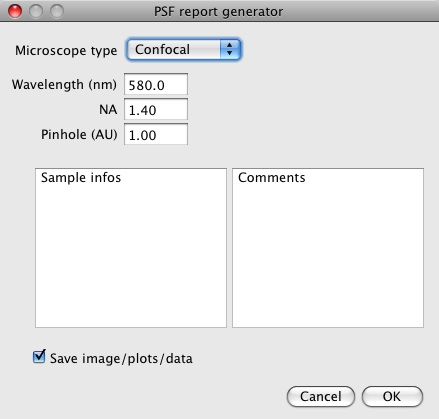
\includegraphics[width=0.35\linewidth]{img/gpr-interf}
				\end{tabular}
			\end{center}
			\caption{\label{fig:gpr-interf}Generate PSF report: the interface.}
		\end{figure} 
	\item Choose the microscope's type, enter the emission wavelength, the numerical aperture of the objective and the pinhole aperture. Sample informations and some comments might also be provided using the appropriate boxes. Ticking the ``Save image/plots/data'' will generate:
	\begin{itemize*}
		\item a jpeg image of the side-views;
		\item three files containing tabulation separated values of the x, y and z profiles (excel files);
		\item a file containing tabulation separated values of the report's summary.
	\end{itemize*}
	\item Click on Ok: a new dialog box appears, inviting the user to choose a folder where all data will be saved;
	\item The pdf report is generated, and appropriate files saved.
\end{enumerate*}

%--------------------------------------------------------------------------------------------------------------------------------------------------------------------
\section{What's on the report ?}
\label{sec:gpr-rep}

The PSF report is composed of two to three pages (see an example of report on fig. \ref{fig:gpr-report}) depending on the informations provided by the user. It is composed of up to 8 sections:
\begin{figure}[!ht]
		\begin{center}
		\begin{tabular}{c}
			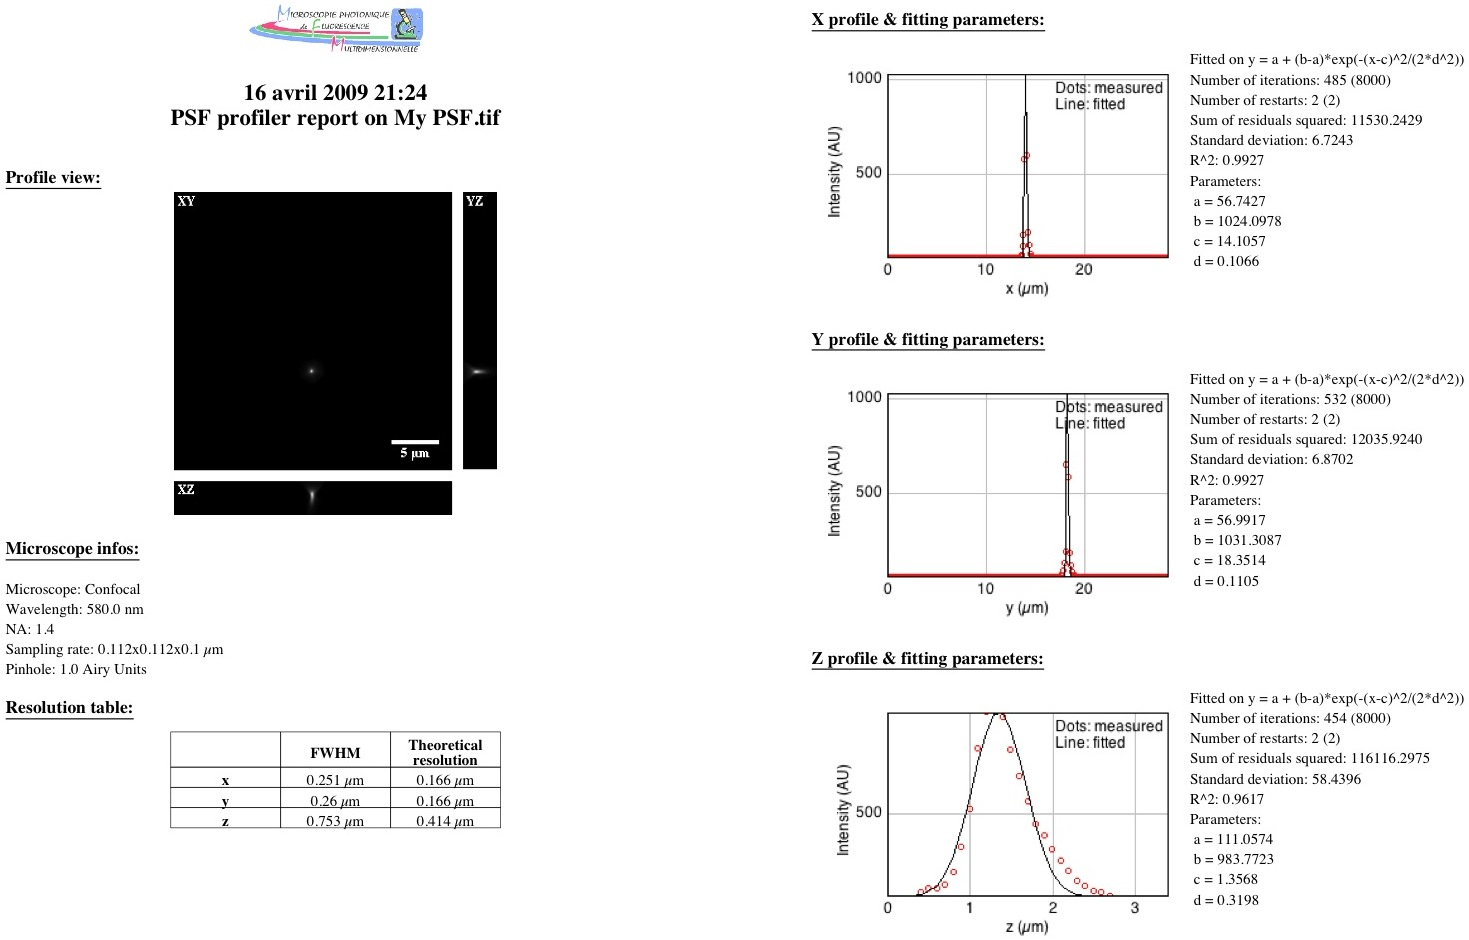
\includegraphics[width=\linewidth]{img/gpr-report}
		\end{tabular}
	\end{center}
	\caption{\label{fig:gpr-report}Generate PSF report: an example of report.}
\end{figure} 
\begin{itemize*}
	\item \textbf{\textit{Profile view}}: image composed of three maximum intensity projections, XY, XZ and YZ;
	\item \textbf{\textit{Microscope infos}}: summarizes informations about the acquisition system and the image's calibration;
	\item \textbf{\textit{Resolution table}}: carries both the resolutions determined by fitting and the theoretical, calculated ones;
	\item \textbf{\textit{x profile and fitting parameters}}: contains a plot of the intensity profile along the x axis and the fitted curve. On the right side of the graph stand the fitting parameters:
		\begin{itemize*}
			\item equation against which the profile is fitted;
			\item number of iterations: self-explanatory;
			\item sum of residuals squared: sum of the differences between the original intensity values and the fitted ones, squared;
			\item standard deviation: standard deviation of the residuals;
			\item the correlation coefficient $R^{2}$ (gives indication on the fitting goodness).
			\item the Gaussian's constants a to d (see \ref{eqn:gpr-gaussian}), c being the position of the beads centre along the x axis;	
		\end{itemize*}
	\item \textbf{\textit{y profile and fitting parameters}}: same as previous along y axis;
	\item \textbf{\textit{z profile and fitting parameters}}: same as previous along z axis;
	\item \textbf{\textit{Sample infos (optional)}}: contains the informations entered by the user in the ``Sample infos'' section of the interface;
	\item \textbf{\textit{Comments (optional)}}: contains the informations entered by the user in the ``Comments'' section of the interface;
\end{itemize*}

%--------------------------------------------------------------------------------------------------------------------------------------------------------------------
\section{Known issues (to date...) and workarounds (if any...)}
\label{sec:gpr-ki}

None...yet.

\mailbug

%%%%%%%%%%%%%%%%%%%%%%%%%%%%%%%%%%%%%%%%%%%%%%%%%%%%%%%%%%%%%
\chapter{Generate axial resolution report}
\label{chap:garr}

%--------------------------------------------------------------------------------------------------------------------------------------------------------------------
\section{How to generate the images ?}
\label{sec:garr-what}

\subsection{Prepare the sample}
\label{sec:garr-proto}

\textit{This sample preparation is aimed at fixing a reflective surface on a slide, overlaid by mounting medium, topped by a coverslip.}

\subsubsection{What do I need ?}
\label{sec:garr-proto-what}

\begin{itemize*}
	\item \textbf{\textit{Single reflector mirror:}} ex: Edmund optics' \href{http://www.edmundoptics.com/onlinecatalog/displayproduct.cfm?productid=1754&showall}{4-6 Wave Mirror 20mm x 20mm Enhanced Aluminum, Ref. NT43-872}.
	\item \textbf{\textit{Ethanol}};
	\item \textbf{\textit{Glue}};
	\item \textbf{\textit{Regular slides}};
	\item \textbf{\textit{Mounting medium}}: should be the same as for the regular, biological samples. Avoid using DAPI containing mounting media. Alternatively, \textbf{\textit{immersion oil}} might also be used as a mounting solution;
	\item \textbf{\textit{Regular coverslips}}: type 1.5 i.e. 0.17mm thick;
	\item \textbf{\textit{Nail polish}}: only in case the mounting solution is not a setting medium.
\end{itemize*}


\subsubsection{How do I do ?}
\label{sec:garr-proto-how}

\begin{enumerate*}
	\item Clean the coverslip, the mirror and the slide using ethanol;
	\item Glue the mirror to the coverslip. Warning: make sure that you glue the glass side of the mirror ! Alternatively, setting mounting medium might be used to stick the mirror on the slide;
	\item Wait for the glue to set;
	\item Mount the coverslip on the slide/mirror by using the mounting medium (or immersion oil). Remove excess of solution by pressing firmly on the coverslip. In case of non setting media, the coverslip should be sealed onto the slide or the mirror (depending on its thickness) using nail polish.
\end{enumerate*}


\subsection{How to acquire the image ?}
\label{sec:garr-flow}

The following chart (see fig. \ref{fig:garr-flowImg}) summarises the procedure for optimal image acquisition, in order to determine the axial resolution on a confocal microscope.

\begin{figure}
	\begin{pdfpic}
		\begin{psmatrix}[colsep=0.4,rowsep=0.425]
			[name=1] \psovalbox[fillstyle=solid, fillcolor=yellow, shadow=true]{\textbf{Begin}}\\
			[name=2] \psframebox[shadow=true]{Set the scanning mode to XZY}\\
			[name=3] \psframebox[shadow=true]{Set the zoom to its maximum}\\
			[name=4] \psframebox[shadow=true]{Fully open the pinhole}\\
			[name=5] \psframebox[shadow=true]{Adjust the laser output to its minimum}\\
			[name=6] \psframebox[shadow=true]{Set the detection to reflexion mode}\\
			[name=7] \psframebox[shadow=true]{Adjust z position}\\
			[name=8] \psdiabox[fillstyle=solid, fillcolor=lightgray, shadow=true]{\begin{tabular}{c}Reflexion plane\\found ?\end{tabular}}\\\\
			[name=9] \psframebox[shadow=true]{Set the pinhole to one Airy unit}\\
			[name=10] \psframebox[shadow=true]{Adjust PMT's gain}\\
			[name=11] \psdiabox[fillstyle=solid, fillcolor=lightgray,shadow=true]{\begin{tabular}{c}Image close\\to saturation ?\end{tabular}}\\\\
			[name=12] \psframebox[shadow=true]{Set the acquisition averaging to 2-4}\\
			[name=13] \psframebox[shadow=true]{Acquire z profile}\\
			[name=14] \psframebox[shadow=true]{Generate the report using MetroloJ}\\
			[name=15] \psovalbox[fillstyle=solid, fillcolor=yellow, shadow=true]{\textbf{End}}
		
			\ncline{->}{1}{2}
			\ncline{->}{2}{3}
			\ncline{->}{3}{4}
			\ncline{->}{4}{5}
			\ncline{->}{5}{6}
			\ncline{->}{6}{7}
			\ncline{->}{7}{8}
			\ncangles[loopsize=1, arm=.5]{->}{8}{7} \aput{:U}{\textbf{No}}
			\ncline{->}{8}{9} \aput{:U}{\textbf{Yes}} 
			\ncline{->}{9}{10}
			\ncline{->}{10}{11}
			\ncangles[loopsize=1, arm=.5]{->}{11}{10} \aput{:U}{\textbf{No}}
			\ncline{->}{11}{12}\aput{:U}{\textbf{Yes}}
			\ncline{->}{12}{13}
			\ncline{->}{13}{14}
			\ncline{->}{14}{15}
		\end{psmatrix}
	\end{pdfpic}
	\caption{\label{fig:garr-flowImg}Flow chart: Image acquisition for axial resolution determination (confocal).}
\end{figure}

%--------------------------------------------------------------------------------------------------------------------------------------------------------------------
\section{What does it do ?}
\label{sec:garr-what}

\begin{enumerate*}
	\item After the user has defined a rectangular ROI, the plugin will generate an average intensity projection of the image along the y axis.
	\item The resulting 1D intensity profile is then fitted to a Gaussian, using the following equation and ImageJ's built-in curve fitting function:
		\begin{equation}
			y = a + (b-a)*e^{\frac{-(x-c)^{2}}{2*d^{2}}}
			\label{eqn:garr-gaussian}
		\end{equation}
	\item The axial resolution i.e. the full-width at half-maximum (FWHM) is calculated as follows, based on the parameters retrieved from the fitting:
	\begin{equation}
		FWHM=2d\sqrt{2ln(2)}
		\label{eqn:garr-FWHM}
	\end{equation}
	\item The theoretical resolutions are calculated as follows, depending on the microscope's type:
		\begin{eqnarray}
			z_{resol, wide-field}=\frac{2*\lambda_{emission}}{NA^2}
			\label{eqn:garr-zWF}\\
			z_{resol, confocal}=\frac{1.4*\lambda_{emission}}{NA^2}
			\label{eqn:garr-zConf}
		\end{eqnarray}
\end{enumerate*}

%--------------------------------------------------------------------------------------------------------------------------------------------------------------------
\section{How to use it ?}
\label{sec:garr-how}

\begin{enumerate*}
	\item Start ImageJ;
	\item Open the image of the z profile;
	\item Launch the plugin by going to Plugins/MetroloJ/Generate axial resolution report
	\item In case the image has not been spatially calibrated, a message error pops up: click on Ok. In the calibration dialog box provide the appropriate values, then re-launch the plugin;
	\item The plugin's interface should appear (see fig. \ref{fig:garr-interf}); 
		\begin{figure}[!ht]
			\begin{center}
				\begin{tabular}{c}
					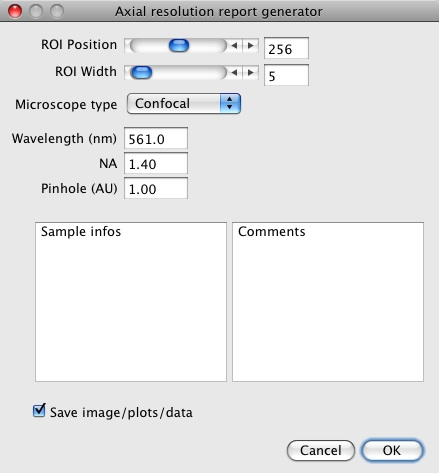
\includegraphics[width=0.35\linewidth]{img/garr-interf}
				\end{tabular}
			\end{center}
			\caption{\label{fig:garr-interf}Generate axial resolution report: the interface.}
		\end{figure} 
	\item Select the position of the ROI and adjust its width;
	\item Choose the microscope's type, enter the emission wavelength, the numerical aperture of the objective and the pinhole aperture. Sample informations and some comments might also be provided using the appropriate boxes. Ticking the ``Save image/plots/data'' will generate:
	\begin{itemize*}
		\item a calibrated jpeg image of the profile, including the ROI's outlines;
		\item a file containing tabulation separated values of the z profile (excel files);
		\item a file containing tabulation separated values of all the numerical data from the report.
	\end{itemize*}
	\item Click on Ok: a new dialog box appears, inviting the user to choose a folder where all data will be saved;
	\item The pdf report is generated, and appropriate files saved.
\end{enumerate*}

%--------------------------------------------------------------------------------------------------------------------------------------------------------------------
\section{What's on the report ?}
\label{sec:garr-rep}

The axial resolution report is composed of two pages (see an example of report on fig. \ref{fig:garr-report}). It is composed of up to 6 sections:
\begin{figure}[!ht]
		\begin{center}
		\begin{tabular}{c}
			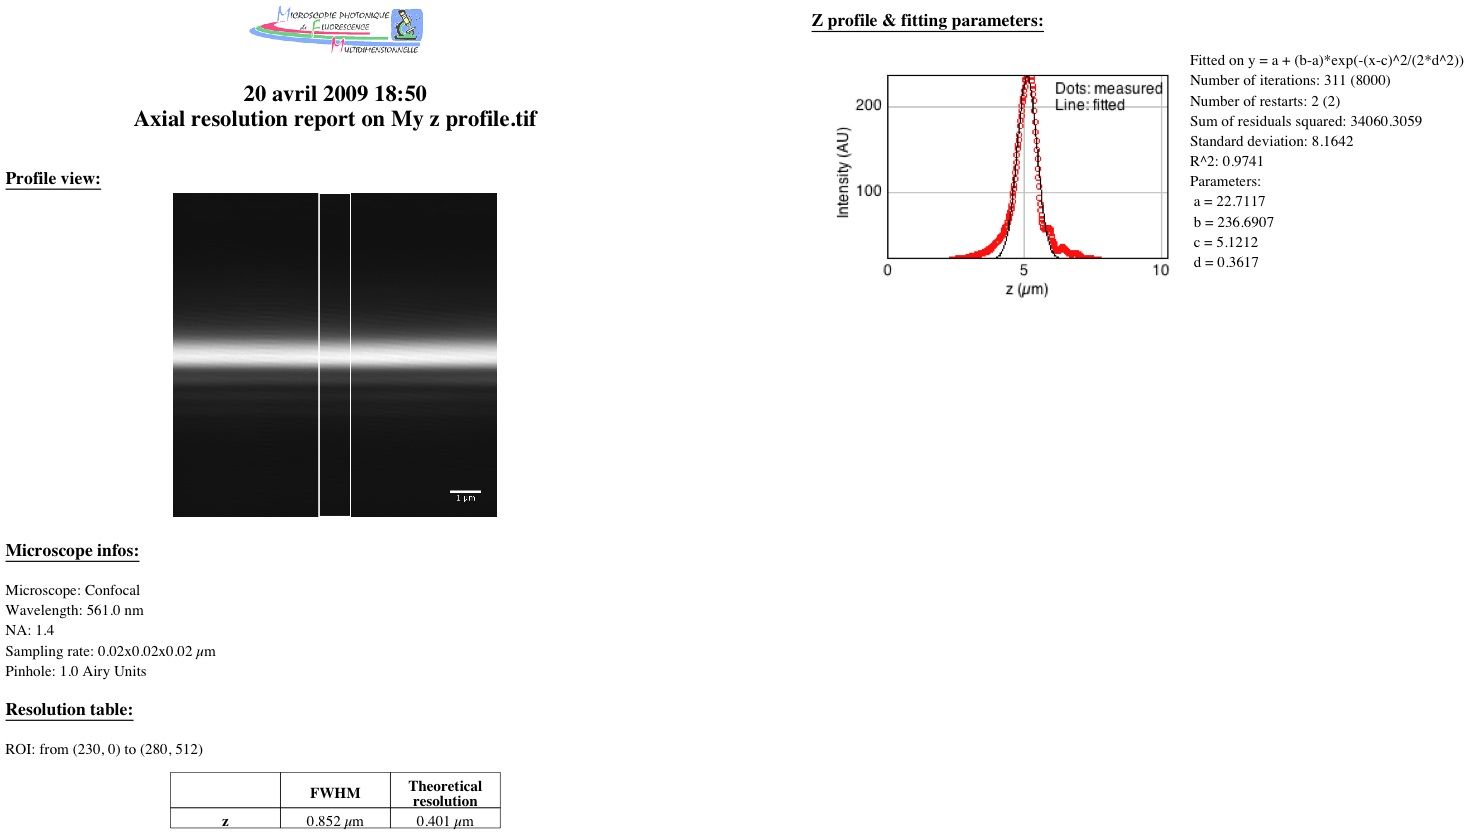
\includegraphics[width=\linewidth]{img/garr-report}
		\end{tabular}
	\end{center}
	\caption{\label{fig:garr-report}Generate axial resolution report: an example of report.}
\end{figure} 
\begin{itemize*}
	\item \textbf{\textit{Profile view}}: a calibrated image of the profile, including the ROI's outlines;
	\item \textbf{\textit{Microscope infos}}: summarizes informations about the acquisition system and the image's calibration;
	\item \textbf{\textit{Resolution table}}: carries both the ROI's position, as well as axial resolutions (experimental and theoretical);;
	\item \textbf{\textit{z profile and fitting parameters}}: contains a plot of the intensity profile along the z axis and the fitted curve. On the right side of the graph stand the fitting parameters:
		\begin{itemize*}
			\item equation against which the profile is fitted;
			\item number of iterations: self-explanatory;
			\item sum of residuals squared: sum of the differences between the original intensity values and the fitted ones, squared;
			\item standard deviation: standard deviation of the residuals;
			\item the correlation coefficient $R^{2}$ (gives indication on the fitting goodness).
			\item the Gaussian's constants a to d (see \ref{eqn:gpr-gaussian}), c being the position of the beads centre along the x axis;	
		\end{itemize*}
	\item \textbf{\textit{Sample infos (optional)}}: contains the informations entered by the user in the ``Sample infos'' section of the interface;
	\item \textbf{\textit{Comments (optional)}}: contains the informations entered by the user in the ``Comments'' section of the interface;
\end{itemize*}


%--------------------------------------------------------------------------------------------------------------------------------------------------------------------
\section{Known issues (to date...) and workarounds (if any...)}
\label{sec:garr-ki}

None...yet.

\mailbug

%%%%%%%%%%%%%%%%%%%%%%%%%%%%%%%%%%%%%%%%%%%%%%%%%%%%%%%%%%%%%
\chapter{Generate co-alignement report}
\label{chap:gcoar}

%--------------------------------------------------------------------------------------------------------------------------------------------------------------------
\section{How to generate the images ?}
\label{sec:gcoar-what}

\subsection{How to prepare the sample ?}
\label{sec:gcoar-proto}

\textit{This sample preparation is aimed at obtaining an array of fluorescent, multi-labelled beads, well appart one from the other, and stably stuck to a coverslip.}

\subsubsection{What do I need ?}
\label{sec:gcoar-proto-what}

\begin{itemize*}
	\item \textbf{\textit{Fluorescent beads:}} their outer diameter should be well above the resolution of the system to test. Two types of beads might be used:
		\begin{itemize*}
			\item Uniformly labelled beads. ex: Molecular Probes' \href{http://probes.invitrogen.com/media/pis/mp07279.pdf}{4$\mu$m TetraSpeck, Ref. T-7283}. However, their diameter is a bit small for low NA objectives...
			\item Non-uniformly labelled beads (inner core carrying one fluorescence, outer ring another). ex: Molecular Probes' \href{http://probes.invitrogen.com/media/pis/mp07234.pdf}{FocalCheck}. 
		\end{itemize*}
	\item \textbf{\textit{Regular slides}};
	\item \textbf{\textit{Regular coverslips}}: type 1.5 i.e. 0.17mm thick, either polylysine coated or not;
	\item If applicable, \textbf{\textit{Poly-L-lysine solution}} (0.1 \% (w/v) in $H_{2}O$) ex: \href{http://www.sigmaaldrich.com/etc/medialib/docs/Sigma/generalinformation2/p8920.Par.0001.File.tmp/p8920.pdf}{Sigma-Aldrich, Ref. P8920};
	\item \textbf{\textit{Ethanol}};
	\item \textbf{\textit{Regular distilled water}};
	\item \textbf{\textit{Mounting medium}}: should be the same as for the regular, biological samples. Avoid using DAPI containing mounting media;
	\item \textbf{\textit{Nail polish}}: only in case the mounting solution is not a setting medium.
\end{itemize*}

\subsubsection{How do I do ?}
\label{sec:gcoar-proto-how}

\begin{enumerate*}
	\item Clean the coverslip and the slide using ethanol;
	\item Dilute the polylysine stock solution to 1/5$^{th}$;
	\item Poor a sufficient amount of the diluted polylysine solution onto the coverslip surface (typically, 200$\mu$l for a 24x24mm coverslip) and leave to coat for 15-30 minutes. The solution hardly covers the full surface, so don't hesitate to use the pipet's tip to force the polylysine into the coverslip's corners; 
	\item Rince the coverslip 2-3 times in distilled water, then drain off the liquid;
	\item Use a vortex to mix the beads' stock suspension;
	\item Dilute the beads suspension in water. Here are some tips and facts:
		\begin{itemize*}
			\item Typically, 200$\mu$l for a 24x24mm coverslip will be requiered;
			\item In general, the beads should not be diluted much from 1/10 to 1/100;
			\item Tests should be done to define the appropriate dilution ratio;
			\item Always vortex the suspensions between and after dilutions;
		\end{itemize*}
	\item Poor a sufficient amount of the diluted beads suspension onto the coverslip surface and leave to sediment for at least 30 minutes. The solution hardly covers the full surface, so don't hesitate to use the pipet's tip to force the suspension into the coverslip's corners; 
	\item Rince the coverslip 2-3 times in distilled water to remove the unattached beads, then drain off the liquid;
	\item Mount the coverslip on the slide by using the mounting medium. In case of non setting media, the coverslip should be sealed onto the slide using nail polish, while avoiding the latter to come under the coverslip.
\end{enumerate*}

NB: Other methods exists in order to produce beads slides, involving dilution in ethanol and leaving the suspension to evaporate. In this case, tests of higher beads dilution might be required. Please note that already prepared beads slides are commercially available (see \href{http://probes.invitrogen.com/media/pis/mp07234.pdf}{FocalCheck Fluorescent Microspheres Size Kit mounted on slide, Ref. F-24633 (6$\mu$m beads) and Ref. F-24634 (15$\mu$m beads)}). However, this kind of preparation doesn't always match with the real \textit{in situ} resolution as the mounting medium might be different from the one used in everyday acquisitions.

\subsection{How to acquire the image ?}
\label{sec:gcoar-flow}

The following chart (see fig. \ref{fig:gcoar-flowImg}) summarises the procedure for optimal image acquisition, in order to determine the co-alignement quality on a confocal microscope.

\begin{figure}
	\begin{pdfpic}
		\begin{psmatrix}[colsep=0.4,rowsep=0.3075]
			[name=1] \psovalbox[fillstyle=solid, fillcolor=yellow, shadow=true]{\textbf{Begin}}\\
			[name=2] \psframebox[shadow=true]{Set the scanning mode to XYZ}\\
			[name=3] \psframebox[shadow=true]{Set the zoom to reach a slight oversampling rate}\\
			[name=4] \psframebox[shadow=true]{Adjust the laser output to its minimum}\\
			[name=5] \psframebox[shadow=true]{Adjust z position}\\
			[name=6] \psdiabox[fillstyle=solid, fillcolor=lightgray, shadow=true]{\begin{tabular}{c}Centre of the\\bead found ?\end{tabular}}\\\\
			[name=7] \psframebox[shadow=true]{Set the acquisition's top and bottom}\\
			[name=8] \psdiabox[fillstyle=solid, fillcolor=lightgray, shadow=true]{\begin{tabular}{c}Stack encompass\\ALL channels ?\end{tabular}}\\\\
			[name=9] \psframebox[shadow=true]{Adjust PMT's gain}\\
			[name=10] \psdiabox[fillstyle=solid, fillcolor=lightgray,shadow=true]{\begin{tabular}{c}Image's centre close\\to saturation ?\end{tabular}}\\\\
			[name=11] \psframebox[shadow=true]{Set the acquisition averaging to 2-4}\\
			[name=12] \psframebox[shadow=true]{Acquire the stack}\\
			[name=13] \psframebox[shadow=true]{Generate the report using MetroloJ}\\
			[name=14] \psovalbox[fillstyle=solid, fillcolor=yellow, shadow=true]{\textbf{End}}
		
			\ncline{->}{1}{2}
			\ncline{->}{2}{3}
			\ncline{->}{3}{4}
			\ncline{->}{4}{5}
			\ncline{->}{5}{6}
			\ncangles[loopsize=1, arm=.5]{->}{6}{5} \aput{:U}{\textbf{No}}
			\ncline{->}{6}{7} \aput{:U}{\textbf{Yes}}
			\ncline{->}{7}{8}
			\ncangles[loopsize=1, arm=.5]{->}{8}{7} \aput{:U}{\textbf{No}}
			\ncline{->}{8}{9} \aput{:U}{\textbf{Yes}} 
			\ncline{->}{9}{10}
			\ncline{->}{10}{11}\aput{:U}{\textbf{Yes}}
			\ncangles[loopsize=1, arm=.5]{->}{10}{9} \aput{:U}{\textbf{No}}
			\ncline{->}{11}{12}
			\ncline{->}{12}{13}
			\ncline{->}{13}{14}
		\end{psmatrix}
	\end{pdfpic}
	\caption{\label{fig:gcoar-flowImg}Acquisition of the image of a multi-labelled bead for co-alignement quality determination (confocal).}
\end{figure}


%--------------------------------------------------------------------------------------------------------------------------------------------------------------------
\section{What does it do ?}
\label{sec:gcoar-what}

\begin{enumerate*}
	\item The plugin will generate two summed intensity projection of the stack along the y and z axes;
	\item On each projection, histogram segmentation is done on the log of intensities, aiming at separating two populations of intensities (background and signal);
	\item Each projection is thresholded is order to highlight the ``signal pixels' population'';
	\item An ellipse is fitted to those pixels (i.e. to the bead's outline), and the coordinates of its centre of mass is determined.
	\item Once all coordinates have been retrieved for each channel, distance between the centre from channel A and centre from channel B is calculated (in fact, all combinaisons of distances are calculated):
	
	\begin{equation}
		dist_{A-B}=\sqrt{(x_{B}-x_{A})^2+(y_{B}-y_{A})^2+(z_{B}-z_{A})^2}
		\label{eqn:gcoar-dist}
	\end{equation}
	
	\item For each couple of coordinates, a reference distance $r_{ref}$ is calculated. This distance is quite easy to determine in 2D as it corresponds to the xy resolution: while considering the centre of the structure on image A, a structure of image B will be co-localized if it is present within a circle traced around centre A of a radius equal to the xy resolution. Due to the disparate resolutions over the three dimensions, this distance is not so easy to calculate in 3D. However, the answer might come from the observation of the factor limiting the resolution: the PSF (Point Spread Function) and more precisely the first Airy disc which might be approximated in 3D as having an ovoid shape (see fig. \ref{fig:gcoar-dist}).
	
	\begin{figure}[!ht]
		\begin{center}
			\begin{tabular}{c}
				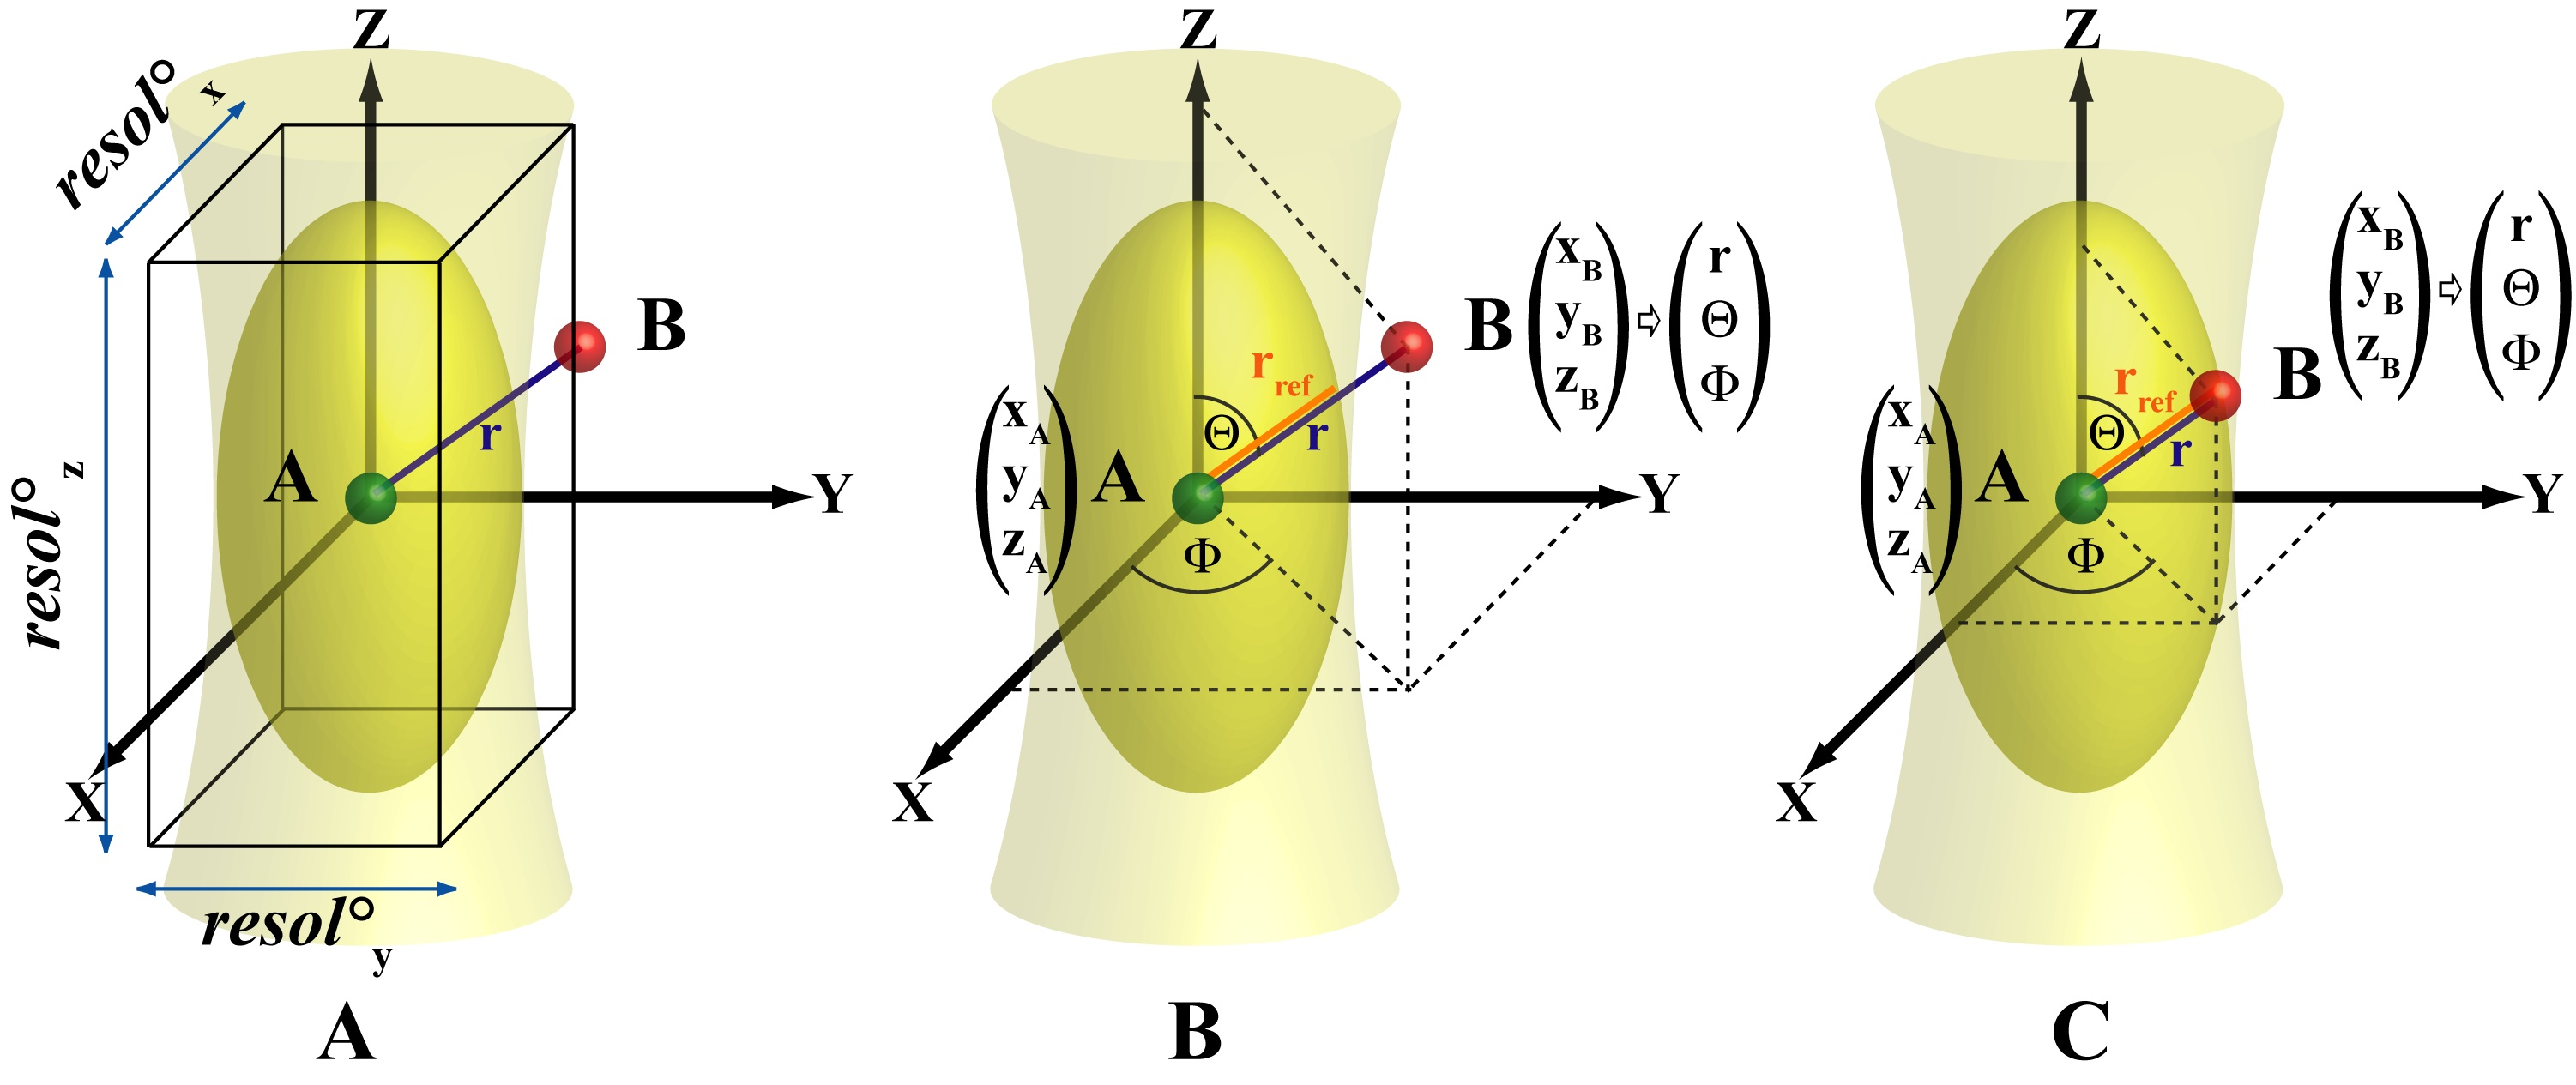
\includegraphics[width=0.9\linewidth]{img/gcoar-dist}
			\end{tabular}
		\end{center}
		\caption{\label{fig:gcoar-dist}Generate co-alignement report: How is the reference distance calculated ? (A) Centres of objects A and B are draw a a red and green sphere, respectively. The PSF is schematised in light yellow, while the first Airy volume appears in dark yellow. The former width, height and depth define the resolution along the 3 axis; (B) A and B are not co-localized as $r>r_{ref}$; (C) A and B are co-localized as $r\le r_{ref}$.\newline
\href{http://imagejdocu.tudor.lu/lib/exe/fetch.php?media=plugin:analysis:jacop_2.0:just_another_colocalization_plugin:jacop_ijconf2008.pdf}{\textit{Illustration from Cordelières and Bolte, ImageJ User and Developper Conference Proceedings, 2008, Luxembourg.}}}
	\end{figure}
	
Therefore in 3D, the reference distance is calculated by considering a reference point and fitting a 3D ellipse around it for which the two characteristic radii correspond to x/y and z resolutions. In this matter changing from Cartesian coordinates to Polar coordinates make it more easy to calculate the reference distance. The two characteristic angles, the azimuth $\Phi$ and the zenith $\Theta$ (see expressions \ref{eqn:gcoar-phi} and \ref{eqn:gcoar-theta}) are first calculated, based on the coordinates of the two centres to analyse. Knowing this orientation, as well as the x, y and z resolutions ($res^\circ_{x}$, $res^\circ_{y}$ and $res^\circ_{z}$ respectively), the distance from the reference centre to the border of the ovoid shape \textbf{$r_{ref}$} is calculated (see expression \ref{eqn:gcoar-refDist}). The inter-centre distance \textbf{$r$} is then compared to this reference distance to assess if co-localization occurs (see fig. \ref{fig:gcoar-dist}C) or not (see fig. \ref{fig:gcoar-dist}B).
	
	\begin{eqnarray}
		\Phi=\arccos\frac{x_{B}-x_{A}}{\sqrt{(x_{B}-x_{A})^2+(y_{B}-y_{A})^2}}\label{eqn:gcoar-phi}\\
		\Theta=\arccos\frac{z_{B}-z_{A}}{\sqrt{(x_{B}-x_{A})^2+(y_{B}-y_{A})^2+(z_{B}-z_{A})^2}}\label{eqn:gcoar-theta}\\
		\xcancel{r_{ref}=\sqrt{(res^\circ_{x}\times\sin\Theta\times\cos\Phi )^2+(res^\circ_{y}\times\sin\Theta\times\sin\Phi)^2+(res^\circ_{z}\times\cos\Theta)^2}\label{eqn:gcoar-refDist}}
	\end{eqnarray}
	
\end{enumerate*}

\textbf{\textcolor{red}{Edit, June 2024}}
\textcolor{red}{As part of the work from QUAREP-LiMi, John Oreopoulos (Oxford Instrument) raised the issue that the above equation is wrong. Checks were made, and external help was reached for. Although the principle of the method stays the same, the above equation should be replaced by the following one:
\begin{ssmall}
	\begin{equation}
   		 r_{ref}=\frac{resol^\circ_{x}\times resol^\circ_{y}\times resol^\circ_{z}}{\sqrt{(resol^\circ_{y} \times resol^\circ_{z} \times\cos\Phi\times\sin\Theta)^2+(resol^\circ_{x}\times resol^\circ_{z} \times\sin\Phi\times\cos\Theta)^2+(resol^\circ_{x}\times resol^\circ_{y} \times\cos\Theta)^2}}
	\end{equation}
\end{ssmall}
}

%--------------------------------------------------------------------------------------------------------------------------------------------------------------------
\section{How to use it ?}
\label{sec:gcoar-how}

\begin{enumerate*}
	\item Start ImageJ;
	\item Open two or three stacks containing exactly one bead;
	\item Launch the plugin by going to Plugins/MetroloJ/Generate co-alignement report
	\item The plugin's interface should appear (see fig. \ref{fig:gcoar-interf}); 
		\begin{figure}[!ht]
			\begin{center}
				\begin{tabular}{c}
					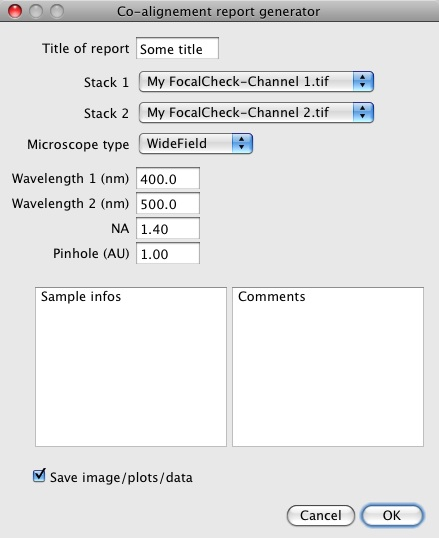
\includegraphics[width=0.35\linewidth]{img/gcoar-interf}
				\end{tabular}
			\end{center}
			\caption{\label{fig:gcoar-interf}Generate co-alignement report: the interface.}
		\end{figure} 
	\item Enter a title for the report, choose which stack should be used for analysis (under ``Stack 3'', ``none'' might also be used), the microscope's type, enter the emission wavelength for each stack, the numerical aperture of the objective and the pinhole aperture. Sample informations and some comments might also be provided using the appropriate boxes. Ticking the ``Save image/plots/data'' will generate:
	\begin{itemize*}
		\item a jpeg image of the side-views;
		\item a file containing tabulation separated values of all the numerical data from the report.
	\end{itemize*}
	\item Click on Ok: a new dialog box appears, inviting the user to choose a folder where all data will be saved;
	\item In case the stack selected under ``Stack 1'' has not been spatially calibrated, a message error pops up: click on Ok. In the calibration dialog box provide the appropriate values, then re-launch the plugin;
	\item The pdf report is generated, and appropriate files saved.
\end{enumerate*}


%--------------------------------------------------------------------------------------------------------------------------------------------------------------------
\section{What's on the report ?}
\label{sec:gcoar-rep}

The co-alignement report is composed of two to three pages (see an example of report on fig. \ref{fig:gcoar-report}) depending on the informations provided by the user. It is composed of up to 7 sections:
\begin{figure}[!ht]
		\begin{center}
		\begin{tabular}{c}
			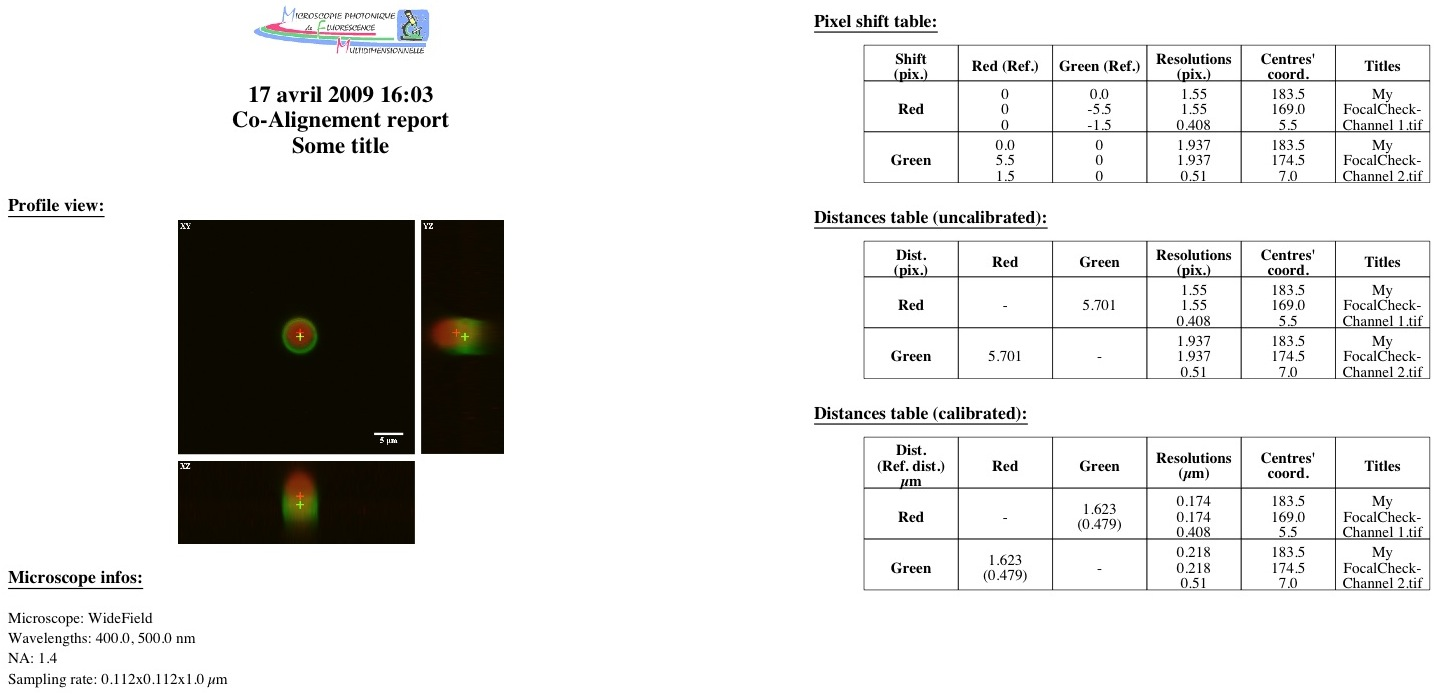
\includegraphics[width=\linewidth]{img/gcoar-report}
		\end{tabular}
	\end{center}
	\caption{\label{fig:gcoar-report}Generate co-alignement report: an example of report.}
\end{figure} 
\begin{itemize*}
	\item \textbf{\textit{Profile view}}: image composed of three maximum intensity projections, XY, XZ and YZ;
	\item \textbf{\textit{Microscope infos}}: summarizes informations about the acquisition system and the image's calibration;
	\item \textbf{\textit{Pixel shift table}}: considering as a reference the channel stated at the beginning of each row, each column show how much pixels separate one channel from the reference along x, y and z axis. This information might be useful to compensate for chromatic aberration using image processing softwares. On each row, resolutions and centre's coordinates are given for the reference channel;
	\item \textbf{\textit{Distance table (uncalibrated)}}: contains distances calculated between two channels, while not taking into account the actual images's calibration;
	\item \textbf{\textit{Distance table (calibrated)}}: contains distances calculated between two channels, while taking into account the actual images's calibration. The distance printed between bracket is the reference distance (see \ref{sec:gcoar-what} and \ref{eqn:gcoar-refDist});
	\item \textbf{\textit{Sample infos (optional)}}: contains the informations entered by the user in the ``Sample infos'' section of the interface;
	\item \textbf{\textit{Comments (optional)}}: contains the informations entered by the user in the ``Comments'' section of the interface;
\end{itemize*}

%--------------------------------------------------------------------------------------------------------------------------------------------------------------------
\section{Known issues (to date...) and workarounds (if any...)}
\label{sec:gcoar-ki}

None...yet.

\mailbug



\end{document}